% Póster A0 vertical (tikzposter). Compilar desde esta carpeta:  latexmk -pdf poster.tex
\documentclass[25pt, a0paper, portrait, margin=0mm, innermargin=14mm, blockverticalspace=14mm,
               colspace=14mm, subcolspace=8mm]{tikzposter}
\usepackage[utf8]{inputenc}
\usepackage[T1]{fontenc}
\usepackage[spanish,es-tabla,es-nodecimaldot]{babel}
\usepackage{amsmath,amssymb}
\usepackage{booktabs}
\usepackage[scaled=0.95]{helvet}
\renewcommand{\familydefault}{\sfdefault}
\usetikzlibrary{arrows.meta,positioning}
\graphicspath{{../figuras/}}
% Generado por analisis.py: NO editar a mano.
\newcommand{\nDatasets}{12}
\newcommand{\nParticiones}{5}
\newcommand{\cambioRL}{$-$14{,}6\,\%}
\newcommand{\dsRL}{11/12}
\newcommand{\pRL}{$0{,}027$}
\newcommand{\pSinHolmRL}{$0{,}003$}
\newcommand{\vsEstRL}{$-$13{,}1\,\%}
\newcommand{\pVsEstRL}{$0{,}027$}
\newcommand{\peorRL}{$+$1{,}2\,\%}
\newcommand{\peorDsRL}{kin8nm}
\newcommand{\cambioKNN}{$-$21{,}2\,\%}
\newcommand{\dsKNN}{9/12}
\newcommand{\pKNN}{$0{,}161$}
\newcommand{\pSinHolmKNN}{$0{,}027$}
\newcommand{\vsEstKNN}{$-$10{,}0\,\%}
\newcommand{\pVsEstKNN}{$0{,}386$}
\newcommand{\peorKNN}{$+$28{,}5\,\%}
\newcommand{\peorDsKNN}{kin8nm}
\newcommand{\cambioArbol}{$-$0{,}6\,\%}
\newcommand{\dsArbol}{5/12}
\newcommand{\pArbol}{$1{,}000$}
\newcommand{\pSinHolmArbol}{$0{,}910$}
\newcommand{\vsEstArbol}{$-$0{,}7\,\%}
\newcommand{\pVsEstArbol}{$1{,}000$}
\newcommand{\peorArbol}{$+$6{,}7\,\%}
\newcommand{\peorDsArbol}{kin8nm}
\newcommand{\cambioRF}{$+$0{,}3\,\%}
\newcommand{\dsRF}{5/12}
\newcommand{\pRF}{$1{,}000$}
\newcommand{\pSinHolmRF}{$0{,}733$}
\newcommand{\vsEstRF}{$+$0{,}3\,\%}
\newcommand{\pVsEstRF}{$1{,}000$}
\newcommand{\peorRF}{$+$12{,}4\,\%}
\newcommand{\peorDsRF}{kin8nm}
\newcommand{\cambioMedio}{$-$9{,}5\,\%}
\newcommand{\sinKinRL}{$-$15{,}9\,\%}
\newcommand{\pSinKinRL}{$0{,}004$}
\newcommand{\sinKinKNN}{$-$24{,}6\,\%}
\newcommand{\pSinKinKNN}{$0{,}021$}
\newcommand{\sinKinArbol}{$-$1{,}3\,\%}
\newcommand{\pSinKinArbol}{$1{,}000$}
\newcommand{\sinKinRF}{$-$0{,}8\,\%}
\newcommand{\pSinKinRF}{$1{,}000$}
\newcommand{\sinKinMedio}{$-$11{,}2\,\%}
\newcommand{\maxRL}{$-$59{,}6\,\%}
\newcommand{\maxDsRL}{cpu\_small}
\newcommand{\maxKNN}{$-$58{,}7\,\%}
\newcommand{\maxDsKNN}{california}
\newcommand{\maxArbol}{$-$9{,}8\,\%}
\newcommand{\maxDsArbol}{space\_ga}
\newcommand{\maxRF}{$-$11{,}7\,\%}
\newcommand{\maxDsRF}{space\_ga}
\newcommand{\maxMaeOrig}{6{,}25}
\newcommand{\maxMaeP}{2{,}52}
\newcommand{\dimMedia}{83\,\%}
\newcommand{\origMedia}{4{,}9}
\newcommand{\compMedia}{2{,}2}
\newcommand{\fracComp}{93\,\%}
\newcommand{\fracElim}{43\,\%}
\newcommand{\siempreMenor}{sí}
\newcommand{\segMediana}{292}
\newcommand{\segMax}{438}
\newcommand{\cribCasos}{14}
\newcommand{\cribP}{0{,}900}
\newcommand{\cribPSeg}{199}
\newcommand{\cribPKNN}{0{,}758}
\newcommand{\cribKnn}{0{,}909}
\newcommand{\cribKnnSeg}{113}
\newcommand{\cribKnnKNN}{0{,}740}
\newcommand{\cribMinimax}{0{,}939}
\newcommand{\cribMinimaxSeg}{234}
\newcommand{\cribMinimaxKNN}{0{,}824}
\newcommand{\cribFamilia}{0{,}893}
\newcommand{\cribFamiliaSeg}{121}
\newcommand{\cribFamiliaKNN}{0{,}740}
\newcommand{\cribParada}{0{,}928}
\newcommand{\cribParadaSeg}{69}
\newcommand{\cribParadaKNN}{0{,}794}
\newcommand{\cribParadaTreinta}{0{,}923}
\newcommand{\cribParadaTreintaSeg}{84}
\newcommand{\cribParadaTreintaKNN}{0{,}794}
\newcommand{\cribSeleccion}{0{,}923}
\newcommand{\cribSeleccionSeg}{95}
\newcommand{\cribSeleccionKNN}{0{,}795}
\newcommand{\ablCasos}{24}
\newcommand{\ablKnn}{$+$1{,}4\,\%}
\newcommand{\ablKnnRL}{$+$12{,}2\,\%}
\newcommand{\ablKnnKNN}{$-$3{,}2\,\%}
\newcommand{\ablKnnArbol}{$-$2{,}1\,\%}
\newcommand{\ablKnnRF}{$-$0{,}5\,\%}
\newcommand{\ablKnnDim}{0{,}83}
\newcommand{\ablSinSint}{$-$0{,}2\,\%}
\newcommand{\ablSinSintRL}{$+$0{,}2\,\%}
\newcommand{\ablSinSintKNN}{$-$1{,}4\,\%}
\newcommand{\ablSinSintArbol}{$+$0{,}5\,\%}
\newcommand{\ablSinSintRF}{$+$0{,}1\,\%}
\newcommand{\ablSinSintDim}{0{,}77}
\newcommand{\ablSinForma}{$+$4{,}1\,\%}
\newcommand{\ablSinFormaRL}{$+$14{,}1\,\%}
\newcommand{\ablSinFormaKNN}{$+$2{,}2\,\%}
\newcommand{\ablSinFormaArbol}{$+$0{,}0\,\%}
\newcommand{\ablSinFormaRF}{$+$0{,}6\,\%}
\newcommand{\ablSinFormaDim}{0{,}75}
\newcommand{\ablSinLimite}{$-$0{,}6\,\%}
\newcommand{\ablSinLimiteRL}{$+$0{,}4\,\%}
\newcommand{\ablSinLimiteKNN}{$-$1{,}3\,\%}
\newcommand{\ablSinLimiteArbol}{$-$1{,}1\,\%}
\newcommand{\ablSinLimiteRF}{$-$0{,}6\,\%}
\newcommand{\ablSinLimiteDim}{1{,}32}
\newcommand{\ablAleat}{$+$3{,}5\,\%}
\newcommand{\ablAleatRL}{$+$4{,}5\,\%}
\newcommand{\ablAleatKNN}{$+$5{,}5\,\%}
\newcommand{\ablAleatArbol}{$+$1{,}9\,\%}
\newcommand{\ablAleatRF}{$+$2{,}1\,\%}
\newcommand{\ablAleatDim}{0{,}82}
\newcommand{\ablAG}{$+$0{,}0\,\%}
\newcommand{\ablAGRL}{$+$0{,}3\,\%}
\newcommand{\ablAGKNN}{$+$0{,}7\,\%}
\newcommand{\ablAGArbol}{$-$0{,}2\,\%}
\newcommand{\ablAGRF}{$-$0{,}7\,\%}
\newcommand{\ablAGDim}{0{,}85}
\newcommand{\rangoP}{3{,}6}
\newcommand{\posP}{1}
\newcommand{\rangoPG}{4{,}0}
\newcommand{\compPGRL}{$-$15{,}7\,\%}
\newcommand{\compPGKNN}{$-$18{,}0\,\%}
\newcommand{\compPGArbol}{$+$0{,}7\,\%}
\newcommand{\compPGRF}{$+$0{,}8\,\%}
\newcommand{\rangoEstPCA}{4{,}1}
\newcommand{\compEstPCARL}{$-$1{,}8\,\%}
\newcommand{\compEstPCAKNN}{$-$12{,}4\,\%}
\newcommand{\compEstPCAArbol}{$-$0{,}6\,\%}
\newcommand{\compEstPCARF}{$-$1{,}9\,\%}
\newcommand{\rangoMLKR}{5{,}2}
\newcommand{\compMLKRRL}{$-$1{,}8\,\%}
\newcommand{\compMLKRKNN}{$-$22{,}5\,\%}
\newcommand{\compMLKRArbol}{$+$2{,}0\,\%}
\newcommand{\compMLKRRF}{$+$2{,}6\,\%}
\newcommand{\rangoPCA}{7{,}2}
\newcommand{\compPCARL}{$+$0{,}6\,\%}
\newcommand{\compPCAKNN}{$-$10{,}4\,\%}
\newcommand{\compPCAArbol}{$+$19{,}3\,\%}
\newcommand{\compPCARF}{$+$17{,}9\,\%}
\newcommand{\rangoYJMV}{4{,}3}
\newcommand{\compYJMVRL}{$+$2{,}4\,\%}
\newcommand{\compYJMVKNN}{$-$14{,}5\,\%}
\newcommand{\compYJMVArbol}{$+$1{,}5\,\%}
\newcommand{\compYJMVRF}{$+$1{,}7\,\%}
% Generado por analisis.py.
\newcommand{\filasPrincipal}{%
R. lineal & 0{,}98 & \textbf{0{,}85} & 11/12 & $0{,}027$ & $-$13{,}1\,\% & $0{,}027$\\
KNN & 0{,}88 & \textbf{0{,}79} & 9/12 & $0{,}161$ & $-$10{,}0\,\% & $0{,}386$\\
Árbol & 1{,}00 & \textbf{0{,}99} & 5/12 & $1{,}000$ & $-$0{,}7\,\% & $1{,}000$\\
RF & 1{,}00 & \textbf{1{,}00} & 5/12 & $1{,}000$ & $+$0{,}3\,\% & $1{,}000$\\
}
\newcommand{\filasDimension}{%
diabetes & 10 & 6{,}2 & 2{,}8 & 9{,}0\\
california & 8 & 5{,}0 & 2{,}0 & 7{,}0\\
concrete & 8 & 5{,}8 & 1{,}0 & 6{,}8\\
stock & 9 & 6{,}4 & 1{,}6 & 8{,}0\\
space\_ga & 6 & 2{,}8 & 2{,}2 & 5{,}0\\
sulfur & 6 & 3{,}0 & 2{,}0 & 5{,}0\\
kin8nm & 8 & 4{,}6 & 2{,}4 & 7{,}0\\
bank8FM & 8 & 3{,}6 & 3{,}4 & 7{,}0\\
puma8NH & 8 & 2{,}2 & 0{,}6 & 2{,}8\\
house\_8L & 8 & 5{,}4 & 1{,}6 & 7{,}0\\
cpu\_small & 12 & 7{,}2 & 3{,}8 & 11{,}0\\
wine\_quality & 11 & 7{,}0 & 3{,}0 & 10{,}0\\
}
\newcommand{\filasCribado}{%
\textbf{$P$: KNN+RL+árbol} & 0{,}91 & 0{,}76 & 0{,}96 & 0{,}99 & 0{,}900 & 0{,}993 & 199\\
fitness solo KNN & 0{,}96 & 0{,}74 & 0{,}97 & 0{,}99 & 0{,}909 & 0{,}992 & 113\\
fitness minimax & 0{,}94 & 0{,}82 & 0{,}99 & 1{,}01 & 0{,}939 & 1{,}012 & 234\\
un fitness por familia & 0{,}90 & 0{,}74 & 0{,}96 & 1{,}00 & 0{,}893 & 1{,}002 & 121\\
+ parada (pac.\ 15) & 0{,}91 & 0{,}79 & 1{,}00 & 1{,}03 & 0{,}928 & 1{,}028 & 69\\
+ parada (pac.\ 30) & 0{,}91 & 0{,}79 & 0{,}99 & 1{,}02 & 0{,}923 & 1{,}022 & 84\\
+ elegir $\theta$ con apartado & 0{,}91 & 0{,}80 & 0{,}99 & 1{,}02 & 0{,}923 & 1{,}021 & 95\\
}
\newcommand{\filasAblacion}{%
fitness solo KNN & $+$12{,}2\,\%$^*$ & $-$3{,}2\,\% & $-$2{,}1\,\% & $-$0{,}5\,\% & $+$1{,}4\,\% & 0{,}83\\
sin síntesis & $+$0{,}2\,\% & $-$1{,}4\,\% & $+$0{,}5\,\% & $+$0{,}1\,\% & $-$0{,}2\,\% & 0{,}77\\
sin forma ($\lambda$ = 1) & $+$14{,}1\,\%$^*$ & $+$2{,}2\,\% & $+$0{,}0\,\% & $+$0{,}6\,\% & $+$4{,}1\,\% & 0{,}75\\
sin límite n$-$1 & $+$0{,}4\,\% & $-$1{,}3\,\% & $-$1{,}1\,\% & $-$0{,}6\,\% & $-$0{,}6\,\% & 1{,}32\\
búsqueda aleatoria & $+$4{,}5\,\%$^*$ & $+$5{,}5\,\% & $+$1{,}9\,\% & $+$2{,}1\,\% & $+$3{,}5\,\% & 0{,}82\\
algoritmo genético & $+$0{,}3\,\% & $+$0{,}7\,\% & $-$0{,}2\,\% & $-$0{,}7\,\% & $+$0{,}0\,\% & 0{,}85\\
}
\newcommand{\filasComparativa}{%
estándar & 0{,}98$^*$ & 0{,}88 & 1{,}00 & 1{,}00 & 4{,}6 & 1{,}00\\
YJ máx.\ verosimilitud & 1{,}02$^*$ & 0{,}85 & 1{,}01 & 1{,}02 & 4{,}3 & 1{,}00\\
cuantiles & 1{,}08$^*$ & 0{,}88 & 1{,}00 & 1{,}00 & 5{,}5 & 1{,}00\\
solo PCA (95\,\%) & 1{,}01$^*$ & 0{,}90 & 1{,}19$^*$ & 1{,}18 & 7{,}2 & 0{,}79\\
solo PCA (\% por VC) & 0{,}99$^*$ & 0{,}88 & 1{,}19$^*$ & 1{,}15 & 6{,}6 & 0{,}91\\
estándar + su PCA & 0{,}98$^*$ & 0{,}88 & 0{,}99 & \textbf{0{,}98} & 4{,}1 & 2{,}00\\
MLKR & 0{,}98$^*$ & \textbf{0{,}78} & 1{,}02 & 1{,}03 & 5{,}2 & 1{,}00\\
prog.\ genética & \textbf{0{,}84} & 0{,}82 & 1{,}01 & 1{,}01 & 4{,}0 & 2{,}00\\
\textbf{$P$} & 0{,}85 & 0{,}79 & \textbf{0{,}99} & 1{,}00 & 3{,}6 & 0{,}83\\
}


\definecolor{uc3mazul}{HTML}{003A70}
\definecolor{uc3mcian}{HTML}{00A6D6}
\definecolor{fondo}{HTML}{F4F7FA}
\definecolor{azulm}{HTML}{2E6DB4}\definecolor{naranjam}{HTML}{D9731A}
\definecolor{verdem}{HTML}{2F9467}\definecolor{grism}{HTML}{5A6772}
\definecolorstyle{uc3m}{}{%
  \colorlet{backgroundcolor}{white}
  \colorlet{framecolor}{uc3mazul}
  \colorlet{titlefgcolor}{white}
  \colorlet{titlebgcolor}{uc3mazul}
  \colorlet{blocktitlebgcolor}{uc3mazul}
  \colorlet{blocktitlefgcolor}{white}
  \colorlet{blockbodybgcolor}{fondo}
  \colorlet{blockbodyfgcolor}{black}
  \colorlet{innerblocktitlebgcolor}{uc3mcian}
  \colorlet{innerblocktitlefgcolor}{white}
  \colorlet{innerblockbodybgcolor}{white}
  \colorlet{innerblockbodyfgcolor}{black}
  \colorlet{notefgcolor}{black}
  \colorlet{notebgcolor}{uc3mcian!15}
  \colorlet{noteframecolor}{uc3mcian}}
\usecolorstyle{uc3m}
\usetitlestyle{Filled}
\useblockstyle{Default}
\settitle{%
  \parbox{\linewidth}{\centering\color{titlefgcolor}\vspace*{16mm}
  {\fontsize{92}{104}\selectfont\bfseries Aumentar, ponderar y reducir\par}\vspace{8mm}
  {\fontsize{50}{60}\selectfont aprendizaje evolutivo de una representación de atributos más pequeña\par}\vspace{12mm}
  {\fontsize{40}{48}\selectfont \@author\par}\vspace{5mm}
  {\fontsize{30}{36}\selectfont \@institute\par}\vspace*{14mm}}}
\title{Aumentar, ponderar y reducir}
\author{Andrea López Salazar}
\institute{IA con inspiración biológica \textbullet\ Máster en Ciencia y Tecnología \textbullet\ Universidad Carlos III de Madrid}

\newcommand{\cifra}[3]{%
  \begin{minipage}[t]{0.48\linewidth}\centering
  {\fontsize{64}{72}\selectfont\bfseries\color{#1}#2}\\[2mm]{\normalsize #3}\end{minipage}}

\begin{document}
\maketitle[width=\paperwidth, roundedcorners=0, linewidth=0, innersep=0mm, titletotopverticalspace=0mm,
           titletoblockverticalspace=14mm]

\begin{columns}
% ===================================================================== columna 1
\column{0.33}
\block{1. El problema}{
Aprender, \textbf{solo con el entrenamiento} y con \textbf{computación evolutiva}, $X\mapsto X'$ con
\textbf{síntesis} de atributos y \textbf{reducción} de la dimensionalidad ($\dim X'<n$), tal que un modelo
\textbf{arbitrario} $M$ entrenado con $X'$ tenga menor MAE: $e'<e$.
\vspace{4mm}

\textbf{La dificultad: ``arbitrario''.} KNN ve la geometría; la R.\ lineal, la forma de cada atributo; un árbol,
invariante a cambios monótonos, solo las \emph{direcciones} por las que corta.
}

\block{2. El método $P$}{
\begin{center}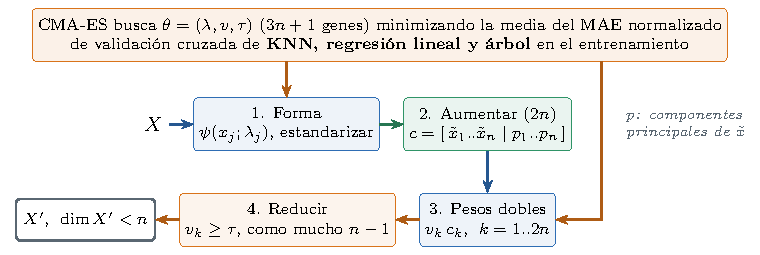
\includegraphics[width=\linewidth]{esquema}\end{center}
\vspace{2mm}
\begin{itemize}
\item \textbf{Aumentar}: $2n$ candidatos = atributos con forma Yeo-Johnson + sus componentes principales
(\textbf{síntesis}).
\item \textbf{Ponderar}: un peso $v_k$ por candidato.
\item \textbf{Reducir}: se conservan los de $v_k\ge\tau$, como mucho $n-1$: $\dim X'<n$ para \emph{todo} individuo.
\textbf{CMA-ES aprende $\tau$}: qué y cuánto se elimina.
\item \textbf{Fitness}: media del MAE normalizado de \textbf{KNN, R.\ lineal y un árbol} (validación cruzada).
\item \textbf{CMA-ES}: $\theta=(\lambda,v,\tau)$, $3n+1$ genes, 1000 evaluaciones.
\end{itemize}
\innerblock{Operadores evolutivos}{\small
Selección por rango de $\mu=\lambda/2$ (robusta al ruido) \textbullet\ recombinación intermedia ponderada
\textbullet\ mutación $\mathcal N(m,\sigma^2C)$ adaptativa (genes acoplados) \textbullet\ reemplazo
$(\mu/\mu_w,\lambda)$ + mejor guardado \textbullet\ restricción por decodificación.}
}

\block{Protocolo}{
\begin{itemize}
\item 12 datasets (diabetes, california + 10 de OpenML). \textbf{Ninguno excluido}.
\item \textbf{Cribado} en semillas de exploración; \textbf{confirmación} en particiones 70/30 nuevas.
\item \textbf{Modelos fijos}: R.\ lineal, KNN, árbol, RF.
\item \textbf{Estadística por dataset} ($n=12$): Wilcoxon + Holm; Friedman + Nemenyi.
\end{itemize}
}

% ===================================================================== columna 2
\column{0.34}
\block{3. Resultado: menos atributos, menos error}{
\cifra{azulm}{\dimMedia}{atributos usados de media \textbullet\ siempre $<n$}\hfill
\cifra{azulm}{\cambioRL}{R. lineal \textbullet\ \dsRL{} datasets \textbullet\ $p$=\pRL}\\[8mm]
\cifra{azulm}{\cambioKNN}{KNN \textbullet\ \dsKNN{} datasets}\hfill
\cifra{grism}{\cambioRF}{Random Forest \textbullet\ árbol \cambioArbol}
\vspace{6mm}

{\small $p$: Wilcoxon por dataset con Holm. Máximo: \maxRL{} (\maxDsRL, R.\ lineal) y \maxKNN{} (\maxDsKNN, KNN).
Caso negativo: \peorDsKNN{} (KNN \peorKNN); sin él, KNN \sinKinKNN.}
\vspace{2mm}
\begin{center}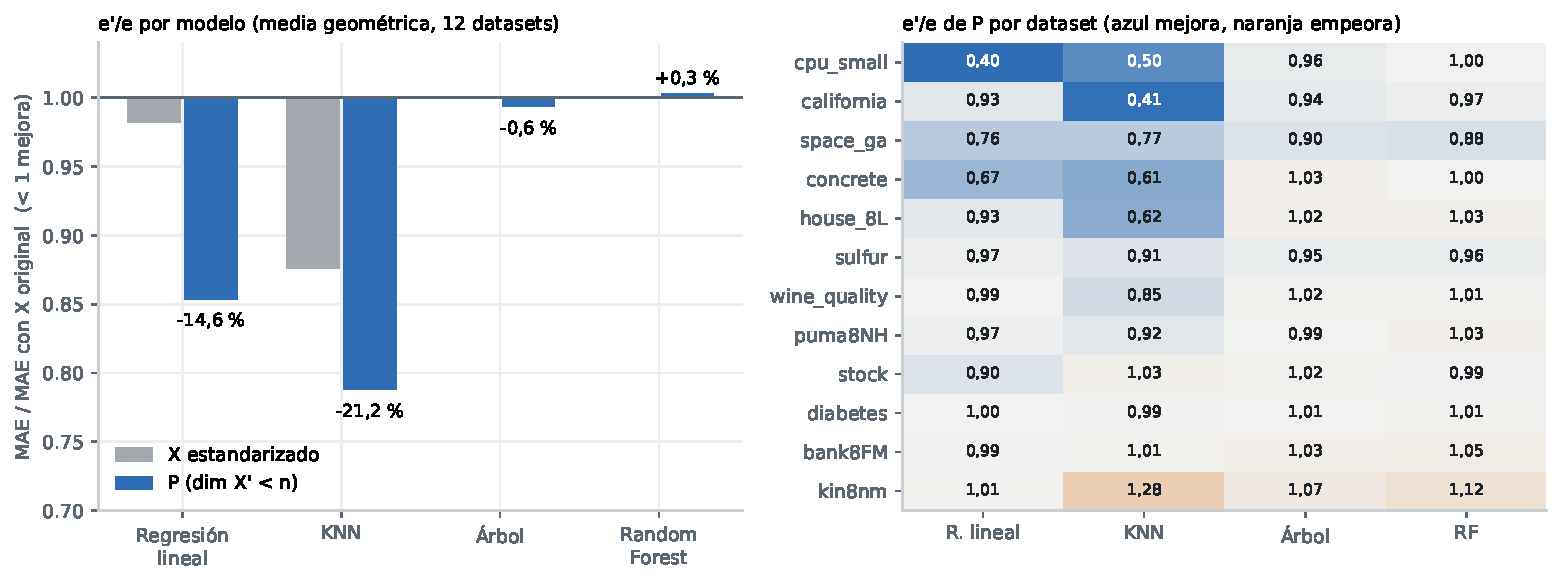
\includegraphics[width=\linewidth]{principal}\end{center}
}

\block{4. Frente a otras ocho transformaciones}{
\begin{center}\small
\begin{tabular}{@{}lcccccc@{}}\toprule
 & R.\,lin. & KNN & Árbol & RF & Rango & $d/n$\\\midrule
\filasComparativa\bottomrule
\end{tabular}\end{center}
{\small $e'/e$; negrita: mejor; $^*$: $P$ mejor con $p<0{,}05$. Rango: Friedman (1 = mejor). $d/n$: $\dim X'/n$.}
\vspace{3mm}

\textbf{Mejor rango medio} (\rangoP) y la única que mejora R.\ lineal y KNN \textbf{reduciendo} la dimensión.
}

% ===================================================================== columna 3
\column{0.33}
\block{5. Cada decisión, contrastada}{
\textbf{Cribado} (exploración): fitness y parada.
\begin{center}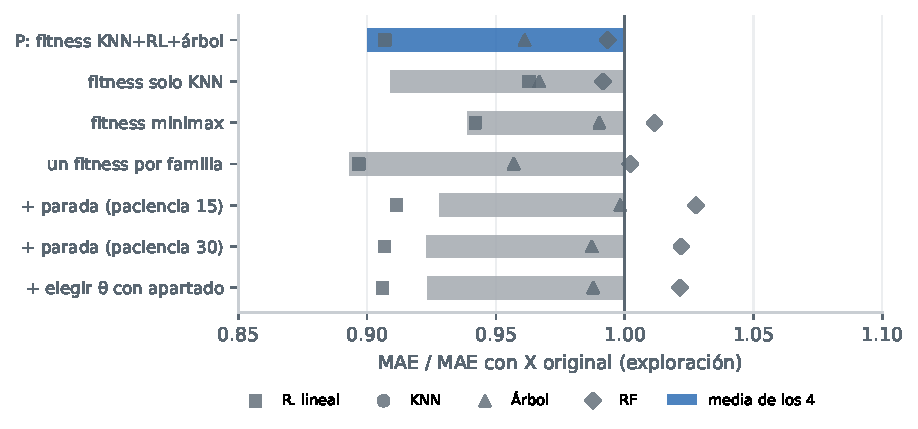
\includegraphics[width=\linewidth]{cribado}\end{center}
{\small Tres familias $>$ solo KNN (\cribP{} vs \cribKnn); minimax y parada por sobreajuste empeoran.}
\vspace{4mm}

\textbf{Ablación} (confirmación): una pieza cada vez.
\begin{center}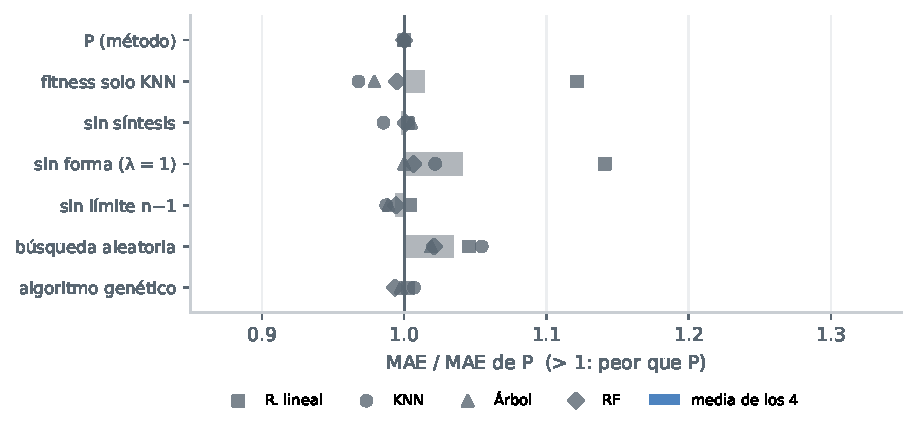
\includegraphics[width=\linewidth]{ablacion}\end{center}
{\small Necesarias: la \textbf{forma} (sin ella, R.\ lineal \ablSinFormaRL$^*$), el \textbf{fitness de tres
familias} (solo KNN: R.\ lineal \ablKnnRL$^*$) y la \textbf{búsqueda evolutiva} (aleatoria: \ablAleat). Un AG empata
con CMA-ES. Sin límite $n-1$ o sin síntesis el error no cambia, pero sin límite $\dim X'=$\,\ablSinLimiteDim\,$n$.
$^*$: $p<0{,}05$ con Holm.}
}

\block{6. Conclusiones}{
\begin{itemize}
\item Cumple \textbf{todos los requisitos}: síntesis, $\dim X'<n$ siempre, criterio de eliminación evolutivo.
\item $e'<e$ en \textbf{R.\ lineal} (significativo) y \textbf{KNN}; árboles sin cambio.
\item \textbf{Mejor rango medio} entre nueve transformaciones.
\item Límites: 12 datasets pequeños; a los árboles les ayuda \emph{añadir} dimensiones.
\end{itemize}
}
\end{columns}
\end{document}
